\documentclass{article}\usepackage[]{graphicx}\usepackage[]{xcolor}
% maxwidth is the original width if it is less than linewidth
% otherwise use linewidth (to make sure the graphics do not exceed the margin)
\makeatletter
\def\maxwidth{ %
  \ifdim\Gin@nat@width>\linewidth
    \linewidth
  \else
    \Gin@nat@width
  \fi
}
\makeatother

\definecolor{fgcolor}{rgb}{0.345, 0.345, 0.345}
\newcommand{\hlnum}[1]{\textcolor[rgb]{0.686,0.059,0.569}{#1}}%
\newcommand{\hlsng}[1]{\textcolor[rgb]{0.192,0.494,0.8}{#1}}%
\newcommand{\hlcom}[1]{\textcolor[rgb]{0.678,0.584,0.686}{\textit{#1}}}%
\newcommand{\hlopt}[1]{\textcolor[rgb]{0,0,0}{#1}}%
\newcommand{\hldef}[1]{\textcolor[rgb]{0.345,0.345,0.345}{#1}}%
\newcommand{\hlkwa}[1]{\textcolor[rgb]{0.161,0.373,0.58}{\textbf{#1}}}%
\newcommand{\hlkwb}[1]{\textcolor[rgb]{0.69,0.353,0.396}{#1}}%
\newcommand{\hlkwc}[1]{\textcolor[rgb]{0.333,0.667,0.333}{#1}}%
\newcommand{\hlkwd}[1]{\textcolor[rgb]{0.737,0.353,0.396}{\textbf{#1}}}%
\let\hlipl\hlkwb

\usepackage{framed}
\makeatletter
\newenvironment{kframe}{%
 \def\at@end@of@kframe{}%
 \ifinner\ifhmode%
  \def\at@end@of@kframe{\end{minipage}}%
  \begin{minipage}{\columnwidth}%
 \fi\fi%
 \def\FrameCommand##1{\hskip\@totalleftmargin \hskip-\fboxsep
 \colorbox{shadecolor}{##1}\hskip-\fboxsep
     % There is no \\@totalrightmargin, so:
     \hskip-\linewidth \hskip-\@totalleftmargin \hskip\columnwidth}%
 \MakeFramed {\advance\hsize-\width
   \@totalleftmargin\z@ \linewidth\hsize
   \@setminipage}}%
 {\par\unskip\endMakeFramed%
 \at@end@of@kframe}
\makeatother

\definecolor{shadecolor}{rgb}{.97, .97, .97}
\definecolor{messagecolor}{rgb}{0, 0, 0}
\definecolor{warningcolor}{rgb}{1, 0, 1}
\definecolor{errorcolor}{rgb}{1, 0, 0}
\newenvironment{knitrout}{}{} % an empty environment to be redefined in TeX

\usepackage{alltt}
\usepackage[margin=1.0in]{geometry} % To set margins
\usepackage{amsmath}  % This allows me to use the align functionality.
                      % If you find yourself trying to replicate
                      % something you found online, ensure you're
                      % loading the necessary packages!
\usepackage{amsfonts} % Math font
\usepackage{fancyvrb}
\usepackage{hyperref} % For including hyperlinks
\usepackage[shortlabels]{enumitem}% For enumerated lists with labels specified
                    % We had to run tlmgr_install("enumitem") in R
\usepackage{float}    % For telling R where to put a table/figure
\usepackage{natbib}        %For the bibliography
\usepackage[skins,breakable]{tcolorbox}        %For the bibliography
\bibliographystyle{apalike}%For the bibliography
\IfFileExists{upquote.sty}{\usepackage{upquote}}{}
\begin{document}
\noindent\textbf{Homework 7: Robust Regression}\\
\noindent\makebox[\linewidth]{\rule{\textwidth}{0.4pt}}
\noindent\underline{Submission Notes:} Please write your answers to each 
question under that question (not altogether at the end). It will be easier for 
me to give full credit if your answer is commented well, including comments 
about where you are completing each sub-part of the question. For an example,
see Homework 1.\\
\noindent\makebox[\linewidth]{\rule{\textwidth}{0.4pt}}


\begin{enumerate}
  %%%%%%%%%%%%%%%%%%%%%%%%%%%%%%%%%%%%%%%%%%%%%%%%%%%%%%%%%%%%%%%%%%%%%%%%%%%%%%
  %%%%%%%%%%%%%%%%%%%%%%%%%%%%%%%%%%%%%%%%%%%%%%%%%%%%%%%%%%%%%%%%%%%%%%%%%%%%%%
  % Question 1
  %%%%%%%%%%%%%%%%%%%%%%%%%%%%%%%%%%%%%%%%%%%%%%%%%%%%%%%%%%%%%%%%%%%%%%%%%%%%%%
  %%%%%%%%%%%%%%%%%%%%%%%%%%%%%%%%%%%%%%%%%%%%%%%%%%%%%%%%%%%%%%%%%%%%%%%%%%%%%%
  \item Below, I simulate data with heteroskedastic error, noting the variance
  is a function of the predictor $x$.
\begin{knitrout}\scriptsize
\definecolor{shadecolor}{rgb}{0.969, 0.969, 0.969}\color{fgcolor}\begin{kframe}
\begin{alltt}
\hlkwd{set.seed}\hldef{(}\hlnum{1933}\hldef{)}
\hldef{x} \hlkwb{<-} \hlnum{1}\hlopt{:}\hlnum{10}
\hldef{(beta0} \hlkwb{<-} \hlkwd{runif}\hldef{(}\hlnum{1}\hldef{,} \hlopt{-}\hlnum{5}\hldef{,} \hlnum{5}\hldef{))}
\end{alltt}
\begin{verbatim}
## [1] 0.08868237
\end{verbatim}
\begin{alltt}
\hldef{(beta1} \hlkwb{<-} \hlkwd{runif}\hldef{(}\hlnum{1}\hldef{,} \hlopt{-}\hlnum{5}\hldef{,} \hlnum{5}\hldef{))}
\end{alltt}
\begin{verbatim}
## [1] -2.116944
\end{verbatim}
\begin{alltt}
\hldef{y} \hlkwb{<-} \hldef{beta0} \hlopt{+} \hldef{beta1} \hlopt{*} \hldef{x} \hlopt{+} \hlkwd{rnorm}\hldef{(}\hlnum{10}\hldef{,} \hlkwc{mean} \hldef{=} \hlnum{0}\hldef{,} \hlkwc{sd} \hldef{= x)}  \hlcom{# Variance is x^2}

\hldef{dat} \hlkwb{<-} \hlkwd{tibble}\hldef{(}\hlkwc{x} \hldef{= x,}
              \hlkwc{y} \hldef{= y)}
\end{alltt}
\end{kframe}
\end{knitrout}
When I fit an OLS model, it doesn't ``pick up" the regression equation.
\begin{knitrout}\scriptsize
\definecolor{shadecolor}{rgb}{0.969, 0.969, 0.969}\color{fgcolor}\begin{kframe}
\begin{alltt}
\hldef{mod.ols} \hlkwb{<-} \hlkwd{lm}\hldef{(y}\hlopt{~}\hldef{x,} \hlkwc{data}\hldef{=dat)}
\hlkwd{summary}\hldef{(mod.ols)}\hlopt{$}\hldef{coefficients}
\end{alltt}
\begin{verbatim}
##               Estimate Std. Error   t value   Pr(>|t|)
## (Intercept) -6.4290175  2.8929497 -2.222305 0.05697684
## x           -0.7669293  0.4662411 -1.644920 0.13860636
\end{verbatim}
\end{kframe}
\end{knitrout}
In Figure \ref{plotq1}, we see that the increased variance almost creates a 
quadratic (if we ignore the observation at $x=10$)
\begin{knitrout}\scriptsize
\definecolor{shadecolor}{rgb}{0.969, 0.969, 0.969}\color{fgcolor}\begin{kframe}
\begin{alltt}
\hlkwd{ggplot}\hldef{(}\hlkwc{data}\hldef{=dat)}\hlopt{+}
  \hlkwd{geom_point}\hldef{(}\hlkwd{aes}\hldef{(}\hlkwc{x}\hldef{=x,} \hlkwc{y}\hldef{=y))}\hlopt{+}
  \hlkwd{theme_bw}\hldef{()} \hlopt{+}
  \hlkwd{geom_abline}\hldef{(}\hlkwd{aes}\hldef{(}\hlkwc{intercept}\hldef{=}\hlkwd{coef}\hldef{(mod.ols)[}\hlnum{1}\hldef{],}
                  \hlkwc{slope}\hldef{=}\hlkwd{coef}\hldef{(mod.ols)[}\hlnum{2}\hldef{],}
                  \hlkwc{color}\hldef{=}\hlsng{"OLS"}\hldef{))}\hlopt{+}
  \hlkwd{geom_abline}\hldef{(}\hlkwd{aes}\hldef{(}\hlkwc{intercept}\hldef{=beta0,}
                  \hlkwc{slope}\hldef{=beta1,}
                  \hlkwc{color}\hldef{=}\hlsng{"Truth"}\hldef{))}\hlopt{+}
  \hlkwd{labs}\hldef{(}\hlkwc{color}\hldef{=}\hlsng{""}\hldef{)}
\end{alltt}
\end{kframe}
\end{knitrout}
\begin{figure}[H]
\centering
\begin{knitrout}
\definecolor{shadecolor}{rgb}{0.969, 0.969, 0.969}\color{fgcolor}

\includegraphics[width=\maxwidth]{figure/unnamed-chunk-4-1} 
\end{knitrout}
\caption{Heteroskedastic regression data generated for Question 1.}\label{plotq1}
\end{figure}
\begin{enumerate}
  \item Conduct a residual and influence analysis on the \texttt{mod.ols}.\\
  \textbf{Note:} The \emph{known} issue may not be obvious.
  
  \begin{figure}[H]
  \centering
  
\begin{knitrout}\scriptsize
\definecolor{shadecolor}{rgb}{0.969, 0.969, 0.969}\color{fgcolor}\begin{kframe}
\begin{alltt}
\hlkwd{source}\hldef{(}\hlsng{"plotResiduals.R"}\hldef{)}
\hlkwd{source}\hldef{(}\hlsng{"plotInfluence.R"}\hldef{)}

\hlkwd{plotResiduals}\hldef{(mod.ols)}
\end{alltt}
\end{kframe}

\includegraphics[width=\maxwidth]{figure/unnamed-chunk-5-1} 
\end{knitrout}
  
  \label{residual.mod}
  \caption{Residual Analysis on \texttt{mod.ols}}
  \end{figure}
  
  \textcolor{red}{If I was analyzing the residuals of this model I would assume there was a non-linear relationship between the predictors and the response variable due to the clear curved pattern in the residuals. The histogram of the residuals looks a little skewed but it's not terrible for 10 observations. The qqplot indicates a potential non-linear relationship with the quadratic looking pattern on the right tail.}
  
  \begin{figure}[H]
  \centering
  
\begin{knitrout}\scriptsize
\definecolor{shadecolor}{rgb}{0.969, 0.969, 0.969}\color{fgcolor}\begin{kframe}
\begin{alltt}
\hlkwd{plotInfluence}\hldef{(mod.ols)}
\end{alltt}
\end{kframe}

\includegraphics[width=\maxwidth]{figure/unnamed-chunk-6-1} 
\end{knitrout}
  
  \label{influence.mod}
  \caption{Influence Analysis on \texttt{mod.ols}}
  \end{figure}
  
  \textcolor{red}{Looking at the influence, the thing that stands out is the clear leverage pattern across observation numbers, which would indicate to me that the leverage is dependent on $x$. The studentized residuals show similar problems to the residuals in Figure: \ref{influence.mod}. Additionally, with there only being 10 observations, several of them having large Cook's d and DFFITs is a bit concerning due to the sheer proportion of potentially high influence points making up a large part of the model.}
  
  \item Fit a weighted least squares (WLS) regression model.
  \begin{enumerate}
    \item Why is $w_i = 1/x_i^2$ a sensible choice for the weights?\\
    \textbf{Hint:} Why is the RMSE $\approx 1$?

\textcolor{red}{In the setup of the regression equation the variance at each point $x$(1:10) is $x^2$, so weighting each point by $\frac{1}{x^2}$ should make each point have an equal weighted variance of 1.}

    
    \item Fit the model with these weights, how does the result change?
    
\begin{knitrout}\scriptsize
\definecolor{shadecolor}{rgb}{0.969, 0.969, 0.969}\color{fgcolor}\begin{kframe}
\begin{alltt}
\hldef{weights} \hlkwb{=} \hlnum{1}\hlopt{/}\hldef{x}\hlopt{^}\hlnum{2}

\hldef{mod_weighted} \hlkwb{<-} \hlkwd{lm}\hldef{(y} \hlopt{~} \hldef{x,} \hlkwc{data} \hldef{= dat,} \hlkwc{weights} \hldef{= weights)}

\hldef{(sum} \hlkwb{<-} \hlkwd{summary}\hldef{(mod_weighted))}
\end{alltt}
\begin{verbatim}
## 
## Call:
## lm(formula = y ~ x, data = dat, weights = weights)
## 
## Weighted Residuals:
##     Min      1Q  Median      3Q     Max 
## -2.0210 -0.6560  0.0217  0.7014  1.4473 
## 
## Coefficients:
##             Estimate Std. Error t value Pr(>|t|)   
## (Intercept)  -1.7035     1.3762  -1.238  0.25088   
## x            -1.8698     0.5418  -3.451  0.00868 **
## ---
## Signif. codes:  0 '***' 0.001 '**' 0.01 '*' 0.05 '.' 0.1 ' ' 1
## 
## Residual standard error: 1.145 on 8 degrees of freedom
## Multiple R-squared:  0.5982,	Adjusted R-squared:  0.548 
## F-statistic: 11.91 on 1 and 8 DF,  p-value: 0.008678
\end{verbatim}
\end{kframe}
\end{knitrout}
 
 \textcolor{red}{Now that we used the weighted model, the coefficent $\beta_1$ associated with $x$ is estimated to be -1.8698 ($p = 0.00868$). This is only a few tenths greater than the true value of $\beta_1 = -2.1169$. The intercept $\beta_0$ is estimated to be -1.7035 while the true $\beta_0$ is 0.0887, indicating that the estimate for the intercept is still quite off. This would probably be better if the data extended more for $x \leq 0$.}
    
    \item Add the WLS line to the scatterplot.
    
    \begin{figure}[H]
    \centering
    
\begin{knitrout}\scriptsize
\definecolor{shadecolor}{rgb}{0.969, 0.969, 0.969}\color{fgcolor}\begin{kframe}
\begin{alltt}
\hldef{betas} \hlkwb{<-} \hldef{sum}\hlopt{$}\hldef{coefficients}
\hldef{beta0_w} \hlkwb{<-} \hldef{betas[}\hlnum{1}\hldef{,}\hlnum{1}\hldef{]}
\hldef{beta1_w} \hlkwb{<-} \hldef{betas[}\hlnum{2}\hldef{,}\hlnum{1}\hldef{]}

\hlkwd{ggplot}\hldef{(}\hlkwc{data}\hldef{=dat)}\hlopt{+}
  \hlkwd{geom_point}\hldef{(}\hlkwd{aes}\hldef{(}\hlkwc{x}\hldef{=x,} \hlkwc{y}\hldef{=y))}\hlopt{+}
  \hlkwd{theme_bw}\hldef{()} \hlopt{+}
  \hlkwd{geom_abline}\hldef{(}\hlkwd{aes}\hldef{(}\hlkwc{intercept}\hldef{=}\hlkwd{coef}\hldef{(mod.ols)[}\hlnum{1}\hldef{],}
              \hlkwc{slope}\hldef{=}\hlkwd{coef}\hldef{(mod.ols)[}\hlnum{2}\hldef{],}
              \hlkwc{color}\hldef{=}\hlsng{"OLS"}\hldef{))}\hlopt{+}
  \hlkwd{geom_abline}\hldef{(}\hlkwd{aes}\hldef{(}\hlkwc{intercept}\hldef{=beta0,}
              \hlkwc{slope}\hldef{=beta1,}
              \hlkwc{color}\hldef{=}\hlsng{"Truth"}\hldef{))}\hlopt{+}
  \hlkwd{geom_abline}\hldef{(}\hlkwd{aes}\hldef{(}\hlkwc{intercept} \hldef{= beta0_w,}
              \hlkwc{slope}\hldef{=beta1_w,}
              \hlkwc{color}\hldef{=}\hlsng{"WLS"}\hldef{))} \hlopt{+}
  \hlkwd{labs}\hldef{(}\hlkwc{color}\hldef{=}\hlsng{""}\hldef{)} \hlopt{+}
  \hlkwd{geom_hline}\hldef{(}\hlkwc{yintercept} \hldef{=} \hlnum{0}\hldef{,} \hlkwc{linetype}\hldef{=}\hlsng{"dashed"}\hldef{)}
\end{alltt}
\end{kframe}

\includegraphics[width=\maxwidth]{figure/unnamed-chunk-8-1} 
\end{knitrout}
    
    \label{new.mod}
    \caption{Scatterplot with Estimated Regression Lines (Updated With Weighted OLS Model)}
    
    \end{figure}
    
    \textcolor{red}{The weighted model worked as intended here, as clearly the WLS regression line is much closer to the truth than the OLS regression line.}
    
  \end{enumerate}
\end{enumerate}
  %%%%%%%%%%%%%%%%%%%%%%%%%%%%%%%%%%%%%%%%%%%%%%%%%%%%%%%%%%%%%%%%%%%%%%%%%%%%%%
  %%%%%%%%%%%%%%%%%%%%%%%%%%%%%%%%%%%%%%%%%%%%%%%%%%%%%%%%%%%%%%%%%%%%%%%%%%%%%%
  % Question 2
  %%%%%%%%%%%%%%%%%%%%%%%%%%%%%%%%%%%%%%%%%%%%%%%%%%%%%%%%%%%%%%%%%%%%%%%%%%%%%%
  %%%%%%%%%%%%%%%%%%%%%%%%%%%%%%%%%%%%%%%%%%%%%%%%%%%%%%%%%%%%%%%%%%%%%%%%%%%%%%
\item Explore fitting a regression model to the data simulated below.
\begin{knitrout}\scriptsize
\definecolor{shadecolor}{rgb}{0.969, 0.969, 0.969}\color{fgcolor}\begin{kframe}
\begin{alltt}
\hldef{n} \hlkwb{<-} \hlnum{50}
\hlkwd{set.seed}\hldef{(}\hlnum{7272}\hldef{)}
\hldef{x} \hlkwb{<-} \hlkwd{sample}\hldef{(}\hlkwc{x}\hldef{=}\hlkwd{seq}\hldef{(}\hlnum{0}\hldef{,}\hlnum{100}\hldef{,}\hlnum{0.01}\hldef{),} \hlkwc{size}\hldef{=n,} \hlkwc{replace}\hldef{=}\hlnum{TRUE}\hldef{)}
\hldef{e} \hlkwb{<-} \hlkwd{rnorm}\hldef{(}\hlkwc{n}\hldef{=}\hlnum{50}\hldef{,} \hlkwc{mean}\hldef{=}\hlnum{0}\hldef{,} \hlkwc{sd}\hldef{=}\hlnum{5}\hldef{)}
\hldef{y} \hlkwb{<-} \hlnum{3.5} \hlopt{+} \hlnum{2.1}\hlopt{*}\hldef{x} \hlopt{+} \hldef{e}

\hldef{first_dat} \hlkwb{<-} \hlkwd{tibble}\hldef{(}\hlkwc{x} \hldef{= x,}
                    \hlkwc{y} \hldef{= y)}

\hlcom{# Add a misbehaved point}
\hldef{x2} \hlkwb{<-} \hlkwd{c}\hldef{(x,} \hlnum{100}\hldef{)}
\hldef{y2} \hlkwb{<-} \hlkwd{c}\hldef{(y,} \hlnum{25}\hldef{)}
\end{alltt}
\end{kframe}
\end{knitrout}
\begin{enumerate}
	\item Fit an OLS model based on \texttt{x} and \texttt{y}. Check the assumptions of the model and interpret the 
	coefficients of the model; are they what you would expect?
	
\begin{knitrout}\scriptsize
\definecolor{shadecolor}{rgb}{0.969, 0.969, 0.969}\color{fgcolor}\begin{kframe}
\begin{alltt}
\hldef{first_mod} \hlkwb{<-} \hlkwd{lm}\hldef{(y} \hlopt{~} \hldef{x,} \hlkwc{data} \hldef{= first_dat)}
\end{alltt}
\end{kframe}
\end{knitrout}
	
	\begin{figure}[H]
	\centering
	
\begin{knitrout}\scriptsize
\definecolor{shadecolor}{rgb}{0.969, 0.969, 0.969}\color{fgcolor}\begin{kframe}
\begin{alltt}
\hldef{first_mod} \hlkwb{<-} \hlkwd{lm}\hldef{(y} \hlopt{~} \hldef{x,} \hlkwc{data} \hldef{= first_dat)}

\hlkwd{plotResiduals}\hldef{(first_mod)}
\end{alltt}
\end{kframe}

\includegraphics[width=\maxwidth]{figure/unnamed-chunk-11-1} 
\end{knitrout}
	
	\label{first.mod.residual}
	\caption{Residual Analysis on \texttt{x} and \texttt{y} OLS model}
	\end{figure}
	
	\textcolor{red}{The residuals look perfect. They're centered at 0 with good normality. The qqplot is very reasonable. Finally, the residuals are indiscriminantly scattered with constant variance.}
	
	\begin{figure}[H]
	\centering
	
\begin{knitrout}\scriptsize
\definecolor{shadecolor}{rgb}{0.969, 0.969, 0.969}\color{fgcolor}\begin{kframe}
\begin{alltt}
\hlkwd{plotInfluence}\hldef{(first_mod)}
\end{alltt}
\end{kframe}
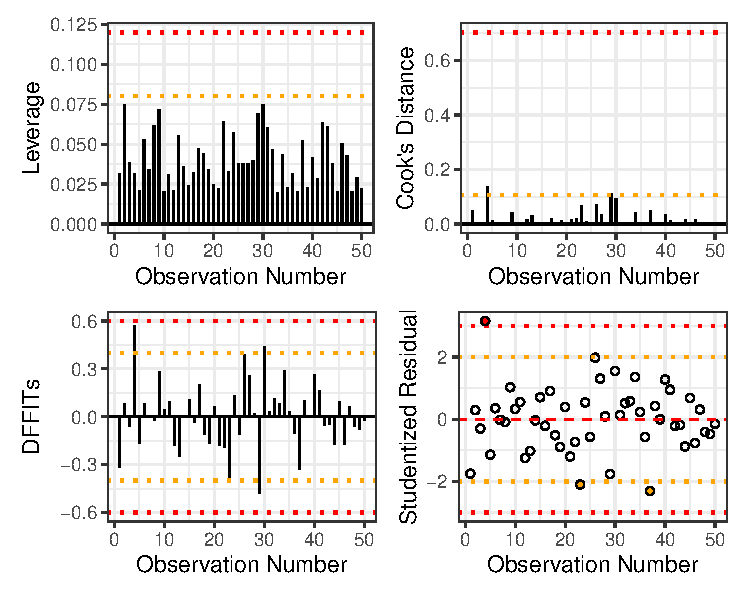
\includegraphics[width=\maxwidth]{figure/unnamed-chunk-12-1} 
\end{knitrout}
	
	\label{first.mod.influence}
	\caption{Influence Analysis on \texttt{x} and \texttt{y} OLS model}
	\end{figure}
	
	\textcolor{red}{The influence analysis on the OLS model looks good as well, with reasonable leverage, DFFITs and Cook's d, with only one point having a potentially unusually high studentized residual (not unusual even for normal, randomized $\epsilon$'s).}
	
\begin{knitrout}\scriptsize
\definecolor{shadecolor}{rgb}{0.969, 0.969, 0.969}\color{fgcolor}\begin{kframe}
\begin{alltt}
\hlkwd{library}\hldef{(xtable)}
\hlkwd{library}\hldef{(effectsize)}

\hldef{first_sum} \hlkwb{<-} \hlkwd{data.frame}\hldef{(}\hlkwd{summary}\hldef{(first_mod)}\hlopt{$}\hldef{coefficients)}

\hlkwd{colnames}\hldef{(first_sum)} \hlkwb{<-} \hlkwd{c}\hldef{(}\hlsng{"Estimate"}\hldef{,} \hlsng{"SE"}\hldef{,} \hlsng{"t"}\hldef{,} \hlsng{"p-value"}\hldef{)}
\hlkwd{rownames}\hldef{(first_sum)} \hlkwb{<-} \hlkwd{c}\hldef{(}\hlsng{"Intercept"}\hldef{,} \hlsng{"x"}\hldef{)}

\hldef{first_sum}\hlopt{$}\hldef{`p-value`} \hlkwb{<-} \hlkwd{ifelse}\hldef{(first_sum}\hlopt{$}\hldef{`p-value`} \hlopt{<} \hlnum{0.001}\hldef{,} \hlsng{"<0.001"}\hldef{, first_sum}\hlopt{$}\hldef{`p-value`)}

\hldef{first_sum} \hlkwb{<-} \hlkwd{xtable}\hldef{(first_sum,}
                    \hlkwc{label} \hldef{=} \hlsng{"first.model.sum"}\hldef{,}
                    \hlkwc{caption} \hldef{=} \hlsng{"OLS Model Summary (Without Outlier)"}\hldef{,}
                    \hlkwc{digits} \hldef{=} \hlnum{3}\hldef{)}
\end{alltt}
\end{kframe}
\end{knitrout}


% latex table generated in R 4.5.1 by xtable 1.8-4 package
% Fri Nov 21 10:33:52 2025
\begin{table}[H]
\centering
\begingroup\normalsize
\begin{tabular}{rrrrl}
  \hline
 & Estimate & SE & t & p-value \\ 
  \hline
Intercept & 5.223 & 1.443 & 3.620 & $<$0.001 \\ 
  x & 2.061 & 0.023 & 87.888 & $<$0.001 \\ 
   \hline
\end{tabular}
\endgroup
\caption{OLS Model Summary (Without Outlier)} 
\label{first.model.sum}
\end{table}



\begin{figure}[H]
\centering

\begin{knitrout}\scriptsize
\definecolor{shadecolor}{rgb}{0.969, 0.969, 0.969}\color{fgcolor}\begin{kframe}
\begin{alltt}
\hlkwd{ggplot}\hldef{(}\hlkwc{data} \hldef{= first_dat,} \hlkwd{aes}\hldef{(}\hlkwc{x} \hldef{= x,} \hlkwc{y} \hldef{= y))} \hlopt{+}
  \hlkwd{geom_point}\hldef{()} \hlopt{+}
  \hlkwd{geom_abline}\hldef{(}\hlkwd{aes}\hldef{(}\hlkwc{intercept} \hldef{= first_sum}\hlopt{$}\hldef{Estimate[}\hlnum{1}\hldef{],}
                  \hlkwc{slope} \hldef{= first_sum}\hlopt{$}\hldef{Estimate[}\hlnum{2}\hldef{],}
                  \hlkwc{color} \hldef{=} \hlsng{"OLS Estimate"}\hldef{))} \hlopt{+}
  \hlkwd{geom_abline}\hldef{(}\hlkwd{aes}\hldef{(}\hlkwc{intercept} \hldef{=} \hlnum{3.5}\hldef{,}
                  \hlkwc{slope} \hldef{=} \hlnum{2.1}\hldef{,}
                  \hlkwc{color} \hldef{=} \hlsng{"True Line"}\hldef{))} \hlopt{+}
  \hlkwd{theme_bw}\hldef{()} \hlopt{+}
  \hlkwd{labs}\hldef{(}\hlkwc{color} \hldef{=} \hlsng{""}\hldef{)} \hlopt{+}
  \hlkwd{geom_hline}\hldef{(}\hlkwc{yintercept} \hldef{=} \hlnum{0}\hldef{,} \hlkwc{linetype} \hldef{=} \hlsng{"dashed"}\hldef{)} \hlopt{+}
  \hlkwd{geom_vline}\hldef{(}\hlkwc{xintercept} \hldef{=} \hlnum{0}\hldef{,} \hlkwc{linetype} \hldef{=} \hlsng{"dashed"}\hldef{)} \hlopt{+}
  \hlkwd{ggtitle}\hldef{(}\hlkwd{bquote}\hldef{(}
  \hlsng{"OLS estimate: "} \hlopt{~}
    \hlkwd{.}\hldef{(}\hlkwd{round}\hldef{(first_sum}\hlopt{$}\hldef{Estimate[}\hlnum{1}\hldef{],} \hlnum{3}\hldef{))} \hlopt{+}
    \hlkwd{.}\hldef{(}\hlkwd{round}\hldef{(first_sum}\hlopt{$}\hldef{Estimate[}\hlnum{2}\hldef{],} \hlnum{3}\hldef{))} \hlopt{*} \hldef{x}
\hldef{))}
\end{alltt}
\end{kframe}

\includegraphics[width=\maxwidth]{figure/unnamed-chunk-15-1} 
\end{knitrout}
	
	\label{first.mod.plot}
	\caption{Scatterplot of the Data with the OLS Regression Line}
	
	\end{figure}
	
	\textcolor{red}{The coefficient for \texttt{x} is very close to the true value. The intercept is reasonably close when looking at the plot. Overall, the two lines are almost visually indistinguishable.}
	
	
	\item Fit an OLS model based on \texttt{x2} and \texttt{y2}. Check the assumptions of the model and interpret the 
	coefficients of the model; are they what you would expect?
\end{enumerate}


\begin{knitrout}\scriptsize
\definecolor{shadecolor}{rgb}{0.969, 0.969, 0.969}\color{fgcolor}\begin{kframe}
\begin{alltt}
\hldef{second_dat} \hlkwb{<-} \hlkwd{tibble}\hldef{(}\hlkwc{x} \hldef{= x2,}
                     \hlkwc{y} \hldef{= y2)}

\hldef{second_mod} \hlkwb{<-} \hlkwd{lm}\hldef{(y} \hlopt{~} \hldef{x,} \hlkwc{data} \hldef{= second_dat)}
\end{alltt}
\end{kframe}
\end{knitrout}
	
	\begin{figure}[H]
	\centering
	
\begin{knitrout}\scriptsize
\definecolor{shadecolor}{rgb}{0.969, 0.969, 0.969}\color{fgcolor}\begin{kframe}
\begin{alltt}
\hlkwd{plotResiduals}\hldef{(second_mod)}
\end{alltt}
\end{kframe}

\includegraphics[width=\maxwidth]{figure/unnamed-chunk-17-1} 
\end{knitrout}
	
	\label{second.mod.residual}
	\caption{Residual Analysis on \texttt{x2} and \texttt{2} OLS model}
	\end{figure}
	

\textcolor{red}{The residuals are pretty hard to analyze here. They're centered around 0 with pretty good normality, just with that huge left tail. We can also see in the qqplot that the data fits perfectly except for the most negative quantile. If we don't focus on the huge outlier, I think the residuals look homoskedastic.}

	
	\begin{figure}[H]
	\centering
	
\begin{knitrout}\scriptsize
\definecolor{shadecolor}{rgb}{0.969, 0.969, 0.969}\color{fgcolor}\begin{kframe}
\begin{alltt}
\hlkwd{plotInfluence}\hldef{(second_mod)}
\end{alltt}
\end{kframe}

\includegraphics[width=\maxwidth]{figure/unnamed-chunk-18-1} 
\end{knitrout}
	
	\label{second.mod.influence}
	\caption{Influence Analysis on \texttt{x2} and \texttt{y2} OLS model}
	\end{figure}
	
	\textcolor{red}{Again, it's quite hard to see everything but besides the huge outlier we don't see any other points on the boundaries of Cook's d, DFFITs, and the studentized residuals. Of course, the $x$ value for our outlier isn't strange so there are no points with concering leverage.}

	
\begin{knitrout}\scriptsize
\definecolor{shadecolor}{rgb}{0.969, 0.969, 0.969}\color{fgcolor}\begin{kframe}
\begin{alltt}
\hldef{second_sum} \hlkwb{<-} \hlkwd{data.frame}\hldef{(}\hlkwd{summary}\hldef{(second_mod)}\hlopt{$}\hldef{coefficients)}

\hlkwd{colnames}\hldef{(second_sum)} \hlkwb{<-} \hlkwd{c}\hldef{(}\hlsng{"Estimate"}\hldef{,} \hlsng{"SE"}\hldef{,} \hlsng{"t"}\hldef{,} \hlsng{"p-value"}\hldef{)}
\hlkwd{rownames}\hldef{(second_sum)} \hlkwb{<-} \hlkwd{c}\hldef{(}\hlsng{"Intercept"}\hldef{,} \hlsng{"x"}\hldef{)}

\hldef{second_sum}\hlopt{$}\hldef{`p-value`} \hlkwb{<-} \hlkwd{ifelse}\hldef{(second_sum}\hlopt{$}\hldef{`p-value`} \hlopt{<} \hlnum{0.001}\hldef{,} \hlsng{"<0.001"}\hldef{,} \hlkwd{round}\hldef{(second_sum}\hlopt{$}\hldef{`p-value`,}\hlnum{3}\hldef{))}

\hldef{second_sum} \hlkwb{<-} \hlkwd{xtable}\hldef{(second_sum,}
                     \hlkwc{label} \hldef{=} \hlsng{"second.model.sum"}\hldef{,}
                     \hlkwc{caption} \hldef{=} \hlsng{"OLS Model Summary (With Outlier)"}\hldef{,}
                     \hlkwc{digits} \hldef{=} \hlnum{3}\hldef{)}
\end{alltt}
\end{kframe}
\end{knitrout}


% latex table generated in R 4.5.1 by xtable 1.8-4 package
% Fri Nov 21 10:33:58 2025
\begin{table}[H]
\centering
\begingroup\normalsize
\begin{tabular}{rrrrl}
  \hline
 & Estimate & SE & t & p-value \\ 
  \hline
Intercept & 10.742 & 7.314 & 1.469 & 0.148 \\ 
  x & 1.891 & 0.117 & 16.160 & $<$0.001 \\ 
   \hline
\end{tabular}
\endgroup
\caption{OLS Model Summary (With Outlier)} 
\label{second.model.sum}
\end{table}



\begin{figure}[H]
\centering

\begin{knitrout}\scriptsize
\definecolor{shadecolor}{rgb}{0.969, 0.969, 0.969}\color{fgcolor}\begin{kframe}
\begin{alltt}
\hlkwd{ggplot}\hldef{(}\hlkwc{data} \hldef{= second_dat,} \hlkwd{aes}\hldef{(}\hlkwc{x} \hldef{= x,} \hlkwc{y} \hldef{= y))} \hlopt{+}
  \hlkwd{geom_point}\hldef{()} \hlopt{+}
  \hlkwd{geom_abline}\hldef{(}\hlkwd{aes}\hldef{(}\hlkwc{intercept} \hldef{= second_sum}\hlopt{$}\hldef{Estimate[}\hlnum{1}\hldef{],}
                  \hlkwc{slope} \hldef{= second_sum}\hlopt{$}\hldef{Estimate[}\hlnum{2}\hldef{],}
                  \hlkwc{color} \hldef{=} \hlsng{"OLS Estimate"}\hldef{))} \hlopt{+}
  \hlkwd{geom_abline}\hldef{(}\hlkwd{aes}\hldef{(}\hlkwc{intercept} \hldef{=} \hlnum{3.5}\hldef{,}
                  \hlkwc{slope} \hldef{=} \hlnum{2.1}\hldef{,}
                  \hlkwc{color} \hldef{=} \hlsng{"True Line"}\hldef{))} \hlopt{+}
  \hlkwd{theme_bw}\hldef{()} \hlopt{+}
  \hlkwd{labs}\hldef{(}\hlkwc{color} \hldef{=} \hlsng{""}\hldef{)} \hlopt{+}
  \hlkwd{geom_hline}\hldef{(}\hlkwc{yintercept} \hldef{=} \hlnum{0}\hldef{,} \hlkwc{linetype} \hldef{=} \hlsng{"dashed"}\hldef{)} \hlopt{+}
  \hlkwd{geom_vline}\hldef{(}\hlkwc{xintercept} \hldef{=} \hlnum{0}\hldef{,} \hlkwc{linetype} \hldef{=} \hlsng{"dashed"}\hldef{)} \hlopt{+}
  \hlkwd{ggtitle}\hldef{(}\hlkwd{bquote}\hldef{(}
  \hlsng{"OLS estimate: "} \hlopt{~}
    \hlkwd{.}\hldef{(}\hlkwd{round}\hldef{(second_sum}\hlopt{$}\hldef{Estimate[}\hlnum{1}\hldef{],} \hlnum{3}\hldef{))} \hlopt{+}
    \hlkwd{.}\hldef{(}\hlkwd{round}\hldef{(second_sum}\hlopt{$}\hldef{Estimate[}\hlnum{2}\hldef{],} \hlnum{3}\hldef{))} \hlopt{*} \hldef{x}
\hldef{))}
\end{alltt}
\end{kframe}

\includegraphics[width=\maxwidth]{figure/unnamed-chunk-21-1} 
\end{knitrout}
	
	\label{second.mod.plot}
	\caption{Scatterplot of the Data with the OLS Regression Line}
	
	\end{figure}
	
	\textcolor{red}{Now that the outlier point is included in the model, the $\beta_1$ estimate for $x$ goes from 2.061 to 1.891, pulling it from the true value of 2.1. Also, the $\beta_0$ estimate of the intercept goes from 5.223 to 10.742, more than doubling and sliding further from the true value of 3.5. We can see those difference in the plot, as the OLS estimate has been dragged down by the outlying point and that makes the OLS estimate worse and worse as $x$ increases.}


  %%%%%%%%%%%%%%%%%%%%%%%%%%%%%%%%%%%%%%%%%%%%%%%%%%%%%%%%%%%%%%%%%%%%%%%%%%%%%%
  %%%%%%%%%%%%%%%%%%%%%%%%%%%%%%%%%%%%%%%%%%%%%%%%%%%%%%%%%%%%%%%%%%%%%%%%%%%%%%
  % Question 3
  %%%%%%%%%%%%%%%%%%%%%%%%%%%%%%%%%%%%%%%%%%%%%%%%%%%%%%%%%%%%%%%%%%%%%%%%%%%%%%
  %%%%%%%%%%%%%%%%%%%%%%%%%%%%%%%%%%%%%%%%%%%%%%%%%%%%%%%%%%%%%%%%%%%%%%%%%%%%%%
\item Continue with Question 2.
\begin{enumerate}
  \item Fit an IRWLS model based on \texttt{x2} and \texttt{y2} using Huber 
  weights. Interpret the coefficients of the model; are they what you would expect?
  
  
\begin{knitrout}\scriptsize
\definecolor{shadecolor}{rgb}{0.969, 0.969, 0.969}\color{fgcolor}\begin{kframe}
\begin{alltt}
\hldef{IWH_mod} \hlkwb{<-} \hldef{MASS}\hlopt{::}\hlkwd{rlm}\hldef{(y} \hlopt{~} \hldef{x,} \hlkwc{data} \hldef{= second_dat,} \hlkwc{psi} \hldef{=} \hlsng{'psi.huber'}\hldef{)}

\hldef{IWH_sum} \hlkwb{<-} \hlkwd{data.frame}\hldef{(}\hlkwd{summary}\hldef{(IWH_mod)}\hlopt{$}\hldef{coefficients)}

\hlkwd{colnames}\hldef{(IWH_sum)} \hlkwb{<-} \hlkwd{c}\hldef{(}\hlsng{"Estimate"}\hldef{,} \hlsng{"SE"}\hldef{,} \hlsng{"t"}\hldef{)}
\hlkwd{rownames}\hldef{(IWH_sum)} \hlkwb{<-} \hlkwd{c}\hldef{(}\hlsng{"Intercept"}\hldef{,} \hlsng{"x"}\hldef{)}

\hldef{IWH_sum} \hlkwb{<-} \hlkwd{xtable}\hldef{(IWH_sum,}
                  \hlkwc{label} \hldef{=} \hlsng{"IWH.model.sum"}\hldef{,}
                  \hlkwc{caption} \hldef{=} \hlsng{"IRLWS Model Summary (With Outlier and Huber Weights)"}\hldef{,}
                  \hlkwc{digits} \hldef{=} \hlnum{3}\hldef{)}
\end{alltt}
\end{kframe}
\end{knitrout}


% latex table generated in R 4.5.1 by xtable 1.8-4 package
% Fri Nov 21 10:33:59 2025
\begin{table}[H]
\centering
\begingroup\normalsize
\begin{tabular}{rrrr}
  \hline
 & Estimate & SE & t \\ 
  \hline
Intercept & 6.039 & 1.422 & 4.246 \\ 
  x & 2.042 & 0.023 & 89.747 \\ 
   \hline
\end{tabular}
\endgroup
\caption{IRLWS Model Summary (With Outlier and Huber Weights)} 
\label{IWH.model.sum}
\end{table}



\begin{figure}[H]
\centering

\begin{knitrout}\scriptsize
\definecolor{shadecolor}{rgb}{0.969, 0.969, 0.969}\color{fgcolor}\begin{kframe}
\begin{alltt}
\hlkwd{ggplot}\hldef{(}\hlkwc{data} \hldef{= second_dat,} \hlkwd{aes}\hldef{(}\hlkwc{x} \hldef{= x,} \hlkwc{y} \hldef{= y))} \hlopt{+}
  \hlkwd{geom_point}\hldef{()} \hlopt{+}
  \hlkwd{geom_abline}\hldef{(}\hlkwd{aes}\hldef{(}\hlkwc{intercept} \hldef{= IWH_sum}\hlopt{$}\hldef{Estimate[}\hlnum{1}\hldef{],}
                  \hlkwc{slope} \hldef{= IWH_sum}\hlopt{$}\hldef{Estimate[}\hlnum{2}\hldef{],}
                  \hlkwc{color} \hldef{=} \hlsng{"Huber IRWLS Estimate"}\hldef{))} \hlopt{+}
  \hlkwd{geom_abline}\hldef{(}\hlkwd{aes}\hldef{(}\hlkwc{intercept} \hldef{=} \hlnum{3.5}\hldef{,}
                  \hlkwc{slope} \hldef{=} \hlnum{2.1}\hldef{,}
                  \hlkwc{color} \hldef{=} \hlsng{"True Line"}\hldef{))} \hlopt{+}
  \hlkwd{theme_bw}\hldef{()} \hlopt{+}
  \hlkwd{labs}\hldef{(}\hlkwc{color} \hldef{=} \hlsng{""}\hldef{)} \hlopt{+}
  \hlkwd{geom_hline}\hldef{(}\hlkwc{yintercept} \hldef{=} \hlnum{0}\hldef{,} \hlkwc{linetype} \hldef{=} \hlsng{"dashed"}\hldef{)} \hlopt{+}
  \hlkwd{geom_vline}\hldef{(}\hlkwc{xintercept} \hldef{=} \hlnum{0}\hldef{,} \hlkwc{linetype} \hldef{=} \hlsng{"dashed"}\hldef{)} \hlopt{+}
  \hlkwd{ggtitle}\hldef{(}\hlkwd{bquote}\hldef{(}
  \hlsng{"Huber IRWLS estimate: "} \hlopt{~}
    \hlkwd{.}\hldef{(}\hlkwd{round}\hldef{(IWH_sum}\hlopt{$}\hldef{Estimate[}\hlnum{1}\hldef{],} \hlnum{3}\hldef{))} \hlopt{+}
    \hlkwd{.}\hldef{(}\hlkwd{round}\hldef{(IWH_sum}\hlopt{$}\hldef{Estimate[}\hlnum{2}\hldef{],} \hlnum{3}\hldef{))} \hlopt{*} \hldef{x}
\hldef{))}
\end{alltt}
\end{kframe}

\includegraphics[width=\maxwidth]{figure/unnamed-chunk-24-1} 
\end{knitrout}
	
	\label{IWH.mod.plot}
	\caption{Scatterplot of the Data with the IRWLS Regression Line (Huber Weights)}
	
	\end{figure}
  
  \textcolor{red}{The IRWLS model with Huber weights $\beta$'s are much closer to the true value than the OLS model. The IRWLS with Huber weights estimate for $\beta_0$ is 6.039 versus the 10.742 of the OLS (true value is 3.5). Also, the $\beta_1$ is 2.042 versus the 1.891 in the OLS model (true value is 2.1). So while the regression is still being pulled down slightly by the outlier, it's noticeable better performing empirically and visually than the standard OLS model.}
  
  \item Fit an IRWLS model based on \texttt{x2} and \texttt{y2} using Bisquare 
  weights. Interpret the coefficients of the model; are they what you would expect?
  
\begin{knitrout}\scriptsize
\definecolor{shadecolor}{rgb}{0.969, 0.969, 0.969}\color{fgcolor}\begin{kframe}
\begin{alltt}
\hldef{IWB_mod} \hlkwb{<-} \hldef{MASS}\hlopt{::}\hlkwd{rlm}\hldef{(y} \hlopt{~} \hldef{x,} \hlkwc{data} \hldef{= second_dat,} \hlkwc{psi} \hldef{=} \hlsng{"psi.bisquare"}\hldef{)}

\hldef{IWB_sum} \hlkwb{<-} \hlkwd{data.frame}\hldef{(}\hlkwd{summary}\hldef{(IWB_mod)}\hlopt{$}\hldef{coefficients)}

\hlkwd{colnames}\hldef{(IWB_sum)} \hlkwb{<-} \hlkwd{c}\hldef{(}\hlsng{"Estimate"}\hldef{,} \hlsng{"SE"}\hldef{,} \hlsng{"t"}\hldef{)}
\hlkwd{rownames}\hldef{(IWB_sum)} \hlkwb{<-} \hlkwd{c}\hldef{(}\hlsng{"Intercept"}\hldef{,} \hlsng{"x"}\hldef{)}

\hldef{IWB_sum} \hlkwb{<-} \hlkwd{xtable}\hldef{(IWB_sum,}
                  \hlkwc{label} \hldef{=} \hlsng{"IWB.model.sum"}\hldef{,}
                  \hlkwc{caption} \hldef{=} \hlsng{"IRLWS Model Summary (With Outlier and Bisquare Weights)"}\hldef{,}
                  \hlkwc{digits} \hldef{=} \hlnum{3}\hldef{)}
\end{alltt}
\end{kframe}
\end{knitrout}


% latex table generated in R 4.5.1 by xtable 1.8-4 package
% Fri Nov 21 10:34:00 2025
\begin{table}[H]
\centering
\begingroup\normalsize
\begin{tabular}{rrrr}
  \hline
 & Estimate & SE & t \\ 
  \hline
Intercept & 5.702 & 1.434 & 3.976 \\ 
  x & 2.050 & 0.023 & 89.372 \\ 
   \hline
\end{tabular}
\endgroup
\caption{IRLWS Model Summary (With Outlier and Bisquare Weights)} 
\label{IWB.model.sum}
\end{table}



\begin{figure}[H]
\centering

\begin{knitrout}\scriptsize
\definecolor{shadecolor}{rgb}{0.969, 0.969, 0.969}\color{fgcolor}\begin{kframe}
\begin{alltt}
\hlkwd{ggplot}\hldef{(}\hlkwc{data} \hldef{= second_dat,} \hlkwd{aes}\hldef{(}\hlkwc{x} \hldef{= x,} \hlkwc{y} \hldef{= y))} \hlopt{+}
  \hlkwd{geom_point}\hldef{()} \hlopt{+}
  \hlkwd{geom_abline}\hldef{(}\hlkwd{aes}\hldef{(}\hlkwc{intercept} \hldef{= IWB_sum}\hlopt{$}\hldef{Estimate[}\hlnum{1}\hldef{],}
                  \hlkwc{slope} \hldef{= IWB_sum}\hlopt{$}\hldef{Estimate[}\hlnum{2}\hldef{],}
                  \hlkwc{color} \hldef{=} \hlsng{"Bisquare IRWLS Estimate"}\hldef{))} \hlopt{+}
  \hlkwd{geom_abline}\hldef{(}\hlkwd{aes}\hldef{(}\hlkwc{intercept} \hldef{=} \hlnum{3.5}\hldef{,}
                  \hlkwc{slope} \hldef{=} \hlnum{2.1}\hldef{,}
                  \hlkwc{color} \hldef{=} \hlsng{"True Line"}\hldef{))} \hlopt{+}
  \hlkwd{theme_bw}\hldef{()} \hlopt{+}
  \hlkwd{labs}\hldef{(}\hlkwc{color} \hldef{=} \hlsng{""}\hldef{)} \hlopt{+}
  \hlkwd{geom_hline}\hldef{(}\hlkwc{yintercept} \hldef{=} \hlnum{0}\hldef{,} \hlkwc{linetype} \hldef{=} \hlsng{"dashed"}\hldef{)} \hlopt{+}
  \hlkwd{geom_vline}\hldef{(}\hlkwc{xintercept} \hldef{=} \hlnum{0}\hldef{,} \hlkwc{linetype} \hldef{=} \hlsng{"dashed"}\hldef{)} \hlopt{+}
  \hlkwd{ggtitle}\hldef{(}\hlkwd{bquote}\hldef{(}
  \hlsng{"Bisquare IRWLS estimate: "} \hlopt{~}
    \hlkwd{.}\hldef{(}\hlkwd{round}\hldef{(IWB_sum}\hlopt{$}\hldef{Estimate[}\hlnum{1}\hldef{],} \hlnum{3}\hldef{))} \hlopt{+}
    \hlkwd{.}\hldef{(}\hlkwd{round}\hldef{(IWB_sum}\hlopt{$}\hldef{Estimate[}\hlnum{2}\hldef{],} \hlnum{3}\hldef{))} \hlopt{*} \hldef{x}
\hldef{))}
\end{alltt}
\end{kframe}
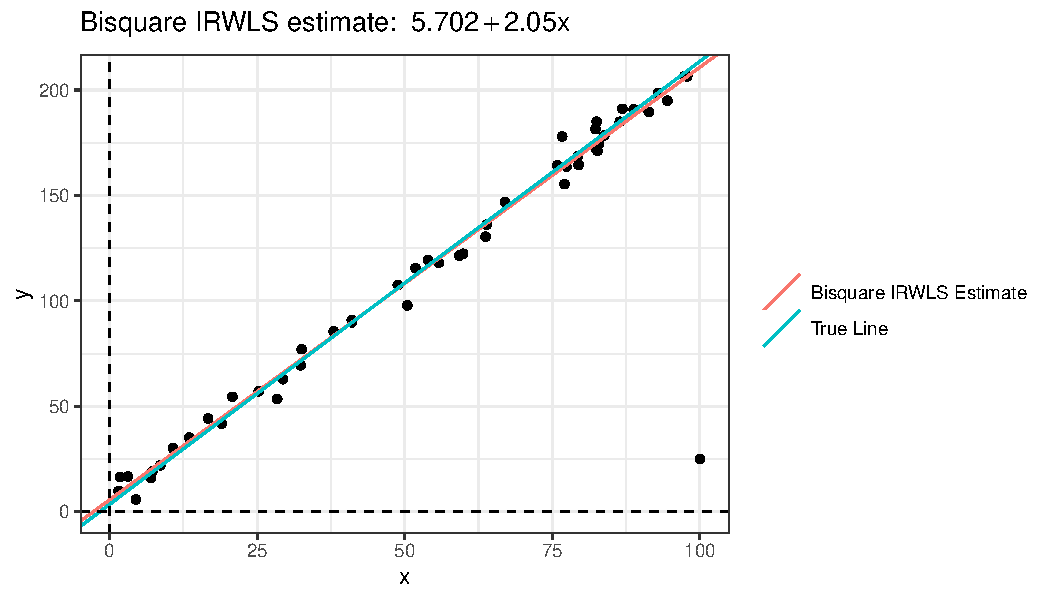
\includegraphics[width=\maxwidth]{figure/unnamed-chunk-27-1} 
\end{knitrout}
	
	\label{IWB.mod.plot}
	\caption{Scatterplot of the Data with the IRWLS Regression Line (Bisquare Weights)}
	
	\end{figure}
	
	\textcolor{red}{The IWRLS model with Bisquare $\beta$'s are also very close to the true values and are very close to the Huber weighted IRWLS. The $\beta_0$ estimate is 5.702 compared to the Huber estimate of 6.039 and the true value of 3.5. The $\beta_1$ estimate is 2.050 compared to the Huber estimate of 2.042 and the true value of 2.1. So in this case, the Bisquare estimates are a tiny bit closer than the Huber estimate.}
  
  
  \item Fit an IRWLS model based on \texttt{x2} and \texttt{y2} using \texttt{lmrob()} 
  from the \texttt{robustbase} package for \texttt{R}. Interpret the coefficients 
  of the model; are they what you would expect?
  
  
\begin{knitrout}\scriptsize
\definecolor{shadecolor}{rgb}{0.969, 0.969, 0.969}\color{fgcolor}\begin{kframe}
\begin{alltt}
\hldef{rob_mod} \hlkwb{<-} \hldef{robustbase}\hlopt{::}\hlkwd{lmrob}\hldef{(y} \hlopt{~} \hldef{x,} \hlkwc{data} \hldef{= second_dat)}

\hldef{rob_sum} \hlkwb{<-} \hlkwd{data.frame}\hldef{(}\hlkwd{summary}\hldef{(rob_mod)}\hlopt{$}\hldef{coefficients)}

\hlkwd{colnames}\hldef{(rob_sum)} \hlkwb{<-} \hlkwd{c}\hldef{(}\hlsng{"Estimate"}\hldef{,} \hlsng{"SE"}\hldef{,} \hlsng{"t"}\hldef{,} \hlsng{"p-value"}\hldef{)}
\hlkwd{rownames}\hldef{(rob_sum)} \hlkwb{<-} \hlkwd{c}\hldef{(}\hlsng{"Intercept"}\hldef{,} \hlsng{"x"}\hldef{)}

\hldef{rob_sum}\hlopt{$}\hldef{`p-value`} \hlkwb{<-} \hlkwd{ifelse}\hldef{(rob_sum}\hlopt{$}\hldef{`p-value`} \hlopt{<} \hlnum{0.001}\hldef{,} \hlsng{"<0.001"}\hldef{,} \hlkwd{round}\hldef{(rob_sum}\hlopt{$}\hldef{`p-value`,}\hlnum{3}\hldef{))}

\hldef{rob_sum} \hlkwb{<-} \hlkwd{xtable}\hldef{(rob_sum,}
                  \hlkwc{label} \hldef{=} \hlsng{"rob.model.sum"}\hldef{,}
                  \hlkwc{caption} \hldef{=} \hlsng{"IRLWS Model Summary (With Outlier and RobustBase Package)"}\hldef{,}
                  \hlkwc{digits} \hldef{=} \hlnum{3}\hldef{)}
\end{alltt}
\end{kframe}
\end{knitrout}


% latex table generated in R 4.5.1 by xtable 1.8-4 package
% Fri Nov 21 10:34:02 2025
\begin{table}[H]
\centering
\begingroup\normalsize
\begin{tabular}{rrrrl}
  \hline
 & Estimate & SE & t & p-value \\ 
  \hline
Intercept & 5.633 & 1.382 & 4.077 & $<$0.001 \\ 
  x & 2.052 & 0.022 & 93.266 & $<$0.001 \\ 
   \hline
\end{tabular}
\endgroup
\caption{IRLWS Model Summary (With Outlier and RobustBase Package)} 
\label{rob.model.sum}
\end{table}



\begin{figure}[H]
\centering

\begin{knitrout}\scriptsize
\definecolor{shadecolor}{rgb}{0.969, 0.969, 0.969}\color{fgcolor}\begin{kframe}
\begin{alltt}
\hlkwd{ggplot}\hldef{(}\hlkwc{data} \hldef{= second_dat,} \hlkwd{aes}\hldef{(}\hlkwc{x} \hldef{= x,} \hlkwc{y} \hldef{= y))} \hlopt{+}
  \hlkwd{geom_point}\hldef{()} \hlopt{+}
  \hlkwd{geom_abline}\hldef{(}\hlkwd{aes}\hldef{(}\hlkwc{intercept} \hldef{= rob_sum}\hlopt{$}\hldef{Estimate[}\hlnum{1}\hldef{],}
                  \hlkwc{slope} \hldef{= rob_sum}\hlopt{$}\hldef{Estimate[}\hlnum{2}\hldef{],}
                  \hlkwc{color} \hldef{=} \hlsng{"RobustBase IRWLS Estimate"}\hldef{))} \hlopt{+}
  \hlkwd{geom_abline}\hldef{(}\hlkwd{aes}\hldef{(}\hlkwc{intercept} \hldef{=} \hlnum{3.5}\hldef{,}
                  \hlkwc{slope} \hldef{=} \hlnum{2.1}\hldef{,}
                  \hlkwc{color} \hldef{=} \hlsng{"True Line"}\hldef{))} \hlopt{+}
  \hlkwd{theme_bw}\hldef{()} \hlopt{+}
  \hlkwd{labs}\hldef{(}\hlkwc{color} \hldef{=} \hlsng{""}\hldef{)} \hlopt{+}
  \hlkwd{geom_hline}\hldef{(}\hlkwc{yintercept} \hldef{=} \hlnum{0}\hldef{,} \hlkwc{linetype} \hldef{=} \hlsng{"dashed"}\hldef{)} \hlopt{+}
  \hlkwd{geom_vline}\hldef{(}\hlkwc{xintercept} \hldef{=} \hlnum{0}\hldef{,} \hlkwc{linetype} \hldef{=} \hlsng{"dashed"}\hldef{)} \hlopt{+}
  \hlkwd{ggtitle}\hldef{(}\hlkwd{bquote}\hldef{(}
  \hlsng{"RobustBase IRWLS estimate: "} \hlopt{~}
    \hlkwd{.}\hldef{(}\hlkwd{round}\hldef{(rob_sum}\hlopt{$}\hldef{Estimate[}\hlnum{1}\hldef{],} \hlnum{3}\hldef{))} \hlopt{+}
    \hlkwd{.}\hldef{(}\hlkwd{round}\hldef{(rob_sum}\hlopt{$}\hldef{Estimate[}\hlnum{2}\hldef{],} \hlnum{3}\hldef{))} \hlopt{*} \hldef{x}
\hldef{))}
\end{alltt}
\end{kframe}
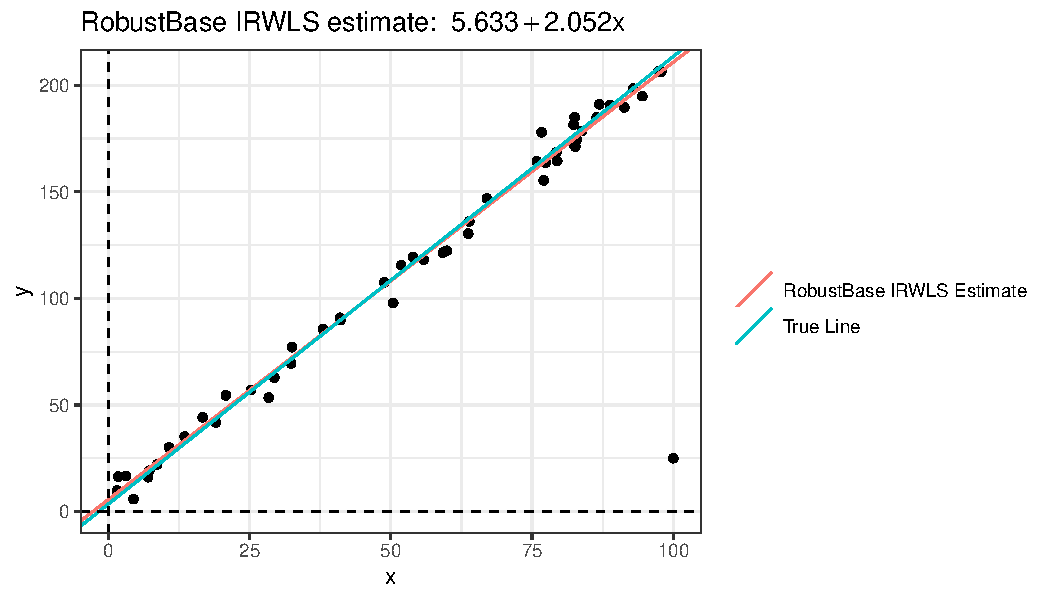
\includegraphics[width=\maxwidth]{figure/unnamed-chunk-30-1} 
\end{knitrout}
	
	\label{rob.mod.plot}
	\caption{Scatterplot of the Data with the IRWLS Regression Line (\texttt{robustbase} package)}
	
	\end{figure}
  
  \textcolor{red}{The $\beta$ estimates are very close to the other weighted methods and fairly close to the true values, with the $\beta_0$ estimate of 5.633 (true value is 3.5) and $\beta_1$ estimate of 2.052 (true value is 2.1).}
  
  
  \item Fit a Quantile regression model based on \texttt{x2} and \texttt{y2}.
  Interpret the coefficients of the model; are they what you would expect?
  
\begin{knitrout}\scriptsize
\definecolor{shadecolor}{rgb}{0.969, 0.969, 0.969}\color{fgcolor}\begin{kframe}
\begin{alltt}
\hldef{quant_mod} \hlkwb{<-} \hldef{quantreg}\hlopt{::}\hlkwd{rq}\hldef{(y} \hlopt{~} \hldef{x,} \hlkwc{data} \hldef{= second_dat,} \hlkwc{tau} \hldef{=} \hlnum{0.5}\hldef{)}

\hldef{quant_sum} \hlkwb{<-} \hlkwd{data.frame}\hldef{(}\hlkwd{summary}\hldef{(quant_mod,} \hlkwc{se} \hldef{=} \hlsng{"boot"}\hldef{)}\hlopt{$}\hldef{coefficients)}

\hlkwd{colnames}\hldef{(quant_sum)} \hlkwb{<-} \hlkwd{c}\hldef{(}\hlsng{"Estimate"}\hldef{,} \hlsng{"SE"}\hldef{,} \hlsng{"t"}\hldef{,} \hlsng{"p-value"}\hldef{)}
\hlkwd{rownames}\hldef{(quant_sum)} \hlkwb{<-} \hlkwd{c}\hldef{(}\hlsng{"Intercept"}\hldef{,} \hlsng{"x"}\hldef{)}

\hldef{quant_sum}\hlopt{$}\hldef{`p-value`} \hlkwb{<-} \hlkwd{ifelse}\hldef{(quant_sum}\hlopt{$}\hldef{`p-value`} \hlopt{<} \hlnum{0.001}\hldef{,} \hlsng{"<0.001"}\hldef{,} \hlkwd{round}\hldef{(quant_sum}\hlopt{$}\hldef{`p-value`,}\hlnum{3}\hldef{))}

\hldef{quant_sum} \hlkwb{<-} \hlkwd{xtable}\hldef{(quant_sum,}
                  \hlkwc{label} \hldef{=} \hlsng{"quant.model.sum"}
                  \hldef{,} \hlkwc{caption} \hldef{=} \hlsng{"Quantile Model Summary (With Outlier)"}
                  \hldef{,} \hlkwc{digits} \hldef{=} \hlnum{3}\hldef{)}
\end{alltt}
\end{kframe}
\end{knitrout}


% latex table generated in R 4.5.1 by xtable 1.8-4 package
% Fri Nov 21 10:34:03 2025
\begin{table}[H]
\centering
\begingroup\normalsize
\begin{tabular}{rrrrl}
  \hline
 & Estimate & SE & t & p-value \\ 
  \hline
Intercept & 5.529 & 1.887 & 2.930 & 0.005 \\ 
  x & 2.053 & 0.029 & 71.055 & $<$0.001 \\ 
   \hline
\end{tabular}
\endgroup
\caption{Quantile Model Summary (With Outlier)} 
\label{quant.model.sum}
\end{table}



\begin{figure}[H]
\centering

\begin{knitrout}\scriptsize
\definecolor{shadecolor}{rgb}{0.969, 0.969, 0.969}\color{fgcolor}\begin{kframe}
\begin{alltt}
\hlkwd{ggplot}\hldef{(}\hlkwc{data} \hldef{= second_dat,} \hlkwd{aes}\hldef{(}\hlkwc{x} \hldef{= x,} \hlkwc{y} \hldef{= y))} \hlopt{+}
  \hlkwd{geom_point}\hldef{()} \hlopt{+}
  \hlkwd{geom_abline}\hldef{(}\hlkwd{aes}\hldef{(}\hlkwc{intercept} \hldef{= quant_sum}\hlopt{$}\hldef{Estimate[}\hlnum{1}\hldef{],}
                  \hlkwc{slope} \hldef{= quant_sum}\hlopt{$}\hldef{Estimate[}\hlnum{2}\hldef{],}
                  \hlkwc{color} \hldef{=} \hlsng{"Quantile Estimate"}\hldef{))} \hlopt{+}
  \hlkwd{geom_abline}\hldef{(}\hlkwd{aes}\hldef{(}\hlkwc{intercept} \hldef{=} \hlnum{3.5}\hldef{,}
                  \hlkwc{slope} \hldef{=} \hlnum{2.1}\hldef{,}
                  \hlkwc{color} \hldef{=} \hlsng{"True Line"}\hldef{))} \hlopt{+}
  \hlkwd{theme_bw}\hldef{()} \hlopt{+}
  \hlkwd{labs}\hldef{(}\hlkwc{color} \hldef{=} \hlsng{""}\hldef{)} \hlopt{+}
  \hlkwd{geom_hline}\hldef{(}\hlkwc{yintercept} \hldef{=} \hlnum{0}\hldef{,} \hlkwc{linetype} \hldef{=} \hlsng{"dashed"}\hldef{)} \hlopt{+}
  \hlkwd{geom_vline}\hldef{(}\hlkwc{xintercept} \hldef{=} \hlnum{0}\hldef{,} \hlkwc{linetype} \hldef{=} \hlsng{"dashed"}\hldef{)} \hlopt{+}
  \hlkwd{ggtitle}\hldef{(}\hlkwd{bquote}\hldef{(}
  \hlsng{"Quantile estimate: "} \hlopt{~}
    \hlkwd{.}\hldef{(}\hlkwd{round}\hldef{(quant_sum}\hlopt{$}\hldef{Estimate[}\hlnum{1}\hldef{],} \hlnum{3}\hldef{))} \hlopt{+}
    \hlkwd{.}\hldef{(}\hlkwd{round}\hldef{(quant_sum}\hlopt{$}\hldef{Estimate[}\hlnum{2}\hldef{],} \hlnum{3}\hldef{))} \hlopt{*} \hldef{x}
\hldef{))}
\end{alltt}
\end{kframe}
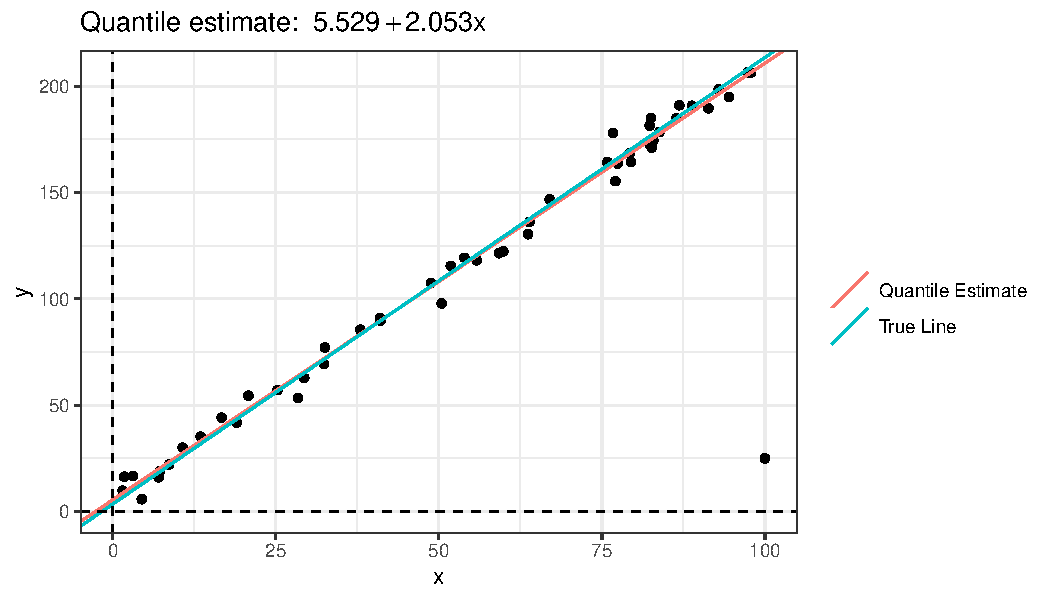
\includegraphics[width=\maxwidth]{figure/unnamed-chunk-33-1} 
\end{knitrout}
	
	\label{quant.mod.plot}
	\caption{Scatterplot of the Data with the Quantile Regression Line}
	
	\end{figure}
	
	\textcolor{red}{The estimates of the $\beta$'s for the quantile regression are very close to the true values: $\beta_0$ = 5.529 (true value is 3.5), $\beta_1$ = 2.053 (true value is 2.1). Visually, the regression lines are very similar as well.}
  
\end{enumerate}
  %%%%%%%%%%%%%%%%%%%%%%%%%%%%%%%%%%%%%%%%%%%%%%%%%%%%%%%%%%%%%%%%%%%%%%%%%%%%%%
  %%%%%%%%%%%%%%%%%%%%%%%%%%%%%%%%%%%%%%%%%%%%%%%%%%%%%%%%%%%%%%%%%%%%%%%%%%%%%%
  % Question 4
  %%%%%%%%%%%%%%%%%%%%%%%%%%%%%%%%%%%%%%%%%%%%%%%%%%%%%%%%%%%%%%%%%%%%%%%%%%%%%%
  %%%%%%%%%%%%%%%%%%%%%%%%%%%%%%%%%%%%%%%%%%%%%%%%%%%%%%%%%%%%%%%%%%%%%%%%%%%%%%
\item \textbf{Optional, but recommended} Plot the results! Create a scatterplot
of \texttt{x2} and \texttt{y2}. Superimpose the true regression line, the OLS
estimate, the IRWLS estimates, and the quantile regression estimate. Interpret
the results.

\begin{figure}[H]
\centering

\begin{knitrout}\scriptsize
\definecolor{shadecolor}{rgb}{0.969, 0.969, 0.969}\color{fgcolor}\begin{kframe}
\begin{alltt}
\hlkwd{ggplot}\hldef{(}\hlkwc{data} \hldef{= second_dat,} \hlkwd{aes}\hldef{(}\hlkwc{x} \hldef{= x,} \hlkwc{y} \hldef{= y))} \hlopt{+}
  \hlkwd{geom_point}\hldef{()} \hlopt{+}
  \hlkwd{geom_abline}\hldef{(}\hlkwd{aes}\hldef{(}\hlkwc{intercept} \hldef{= second_sum}\hlopt{$}\hldef{Estimate[}\hlnum{1}\hldef{],}
                  \hlkwc{slope} \hldef{= second_sum}\hlopt{$}\hldef{Estimate[}\hlnum{2}\hldef{],}
                  \hlkwc{color} \hldef{=} \hlsng{"OLS"}\hldef{))} \hlopt{+}
  \hlkwd{geom_abline}\hldef{(}\hlkwd{aes}\hldef{(}\hlkwc{intercept} \hldef{= IWH_sum}\hlopt{$}\hldef{Estimate[}\hlnum{1}\hldef{],}
                  \hlkwc{slope} \hldef{= IWH_sum}\hlopt{$}\hldef{Estimate[}\hlnum{2}\hldef{],}
                  \hlkwc{color} \hldef{=} \hlsng{"Huber IRWLS"}\hldef{))} \hlopt{+}
  \hlkwd{geom_abline}\hldef{(}\hlkwd{aes}\hldef{(}\hlkwc{intercept} \hldef{= IWB_sum}\hlopt{$}\hldef{Estimate[}\hlnum{1}\hldef{],}
                  \hlkwc{slope} \hldef{= IWB_sum}\hlopt{$}\hldef{Estimate[}\hlnum{2}\hldef{],}
                  \hlkwc{color} \hldef{=} \hlsng{"Bisquare IRWLS"}\hldef{))} \hlopt{+}
  \hlkwd{geom_abline}\hldef{(}\hlkwd{aes}\hldef{(}\hlkwc{intercept} \hldef{= rob_sum}\hlopt{$}\hldef{Estimate[}\hlnum{1}\hldef{],}
                  \hlkwc{slope} \hldef{= rob_sum}\hlopt{$}\hldef{Estimate[}\hlnum{2}\hldef{],}
                  \hlkwc{color} \hldef{=} \hlsng{"RobustBase IRWLS"}\hldef{))} \hlopt{+}
  \hlkwd{geom_abline}\hldef{(}\hlkwd{aes}\hldef{(}\hlkwc{intercept} \hldef{= quant_sum}\hlopt{$}\hldef{Estimate[}\hlnum{1}\hldef{],}
                  \hlkwc{slope} \hldef{= quant_sum}\hlopt{$}\hldef{Estimate[}\hlnum{2}\hldef{],}
                  \hlkwc{color} \hldef{=} \hlsng{"Quantile"}\hldef{))} \hlopt{+}
  \hlkwd{geom_abline}\hldef{(}\hlkwd{aes}\hldef{(}\hlkwc{intercept} \hldef{=} \hlnum{3.5}\hldef{,}
                  \hlkwc{slope} \hldef{=} \hlnum{2.1}\hldef{,}
                  \hlkwc{color} \hldef{=} \hlsng{"True Line"}\hldef{))} \hlopt{+}
  \hlkwd{theme_bw}\hldef{()} \hlopt{+}
  \hlkwd{labs}\hldef{(}\hlkwc{color} \hldef{=} \hlsng{""}\hldef{)} \hlopt{+}
  \hlkwd{geom_hline}\hldef{(}\hlkwc{yintercept} \hldef{=} \hlnum{0}\hldef{,} \hlkwc{linetype} \hldef{=} \hlsng{"dashed"}\hldef{)} \hlopt{+}
  \hlkwd{geom_vline}\hldef{(}\hlkwc{xintercept} \hldef{=} \hlnum{0}\hldef{,} \hlkwc{linetype} \hldef{=} \hlsng{"dashed"}\hldef{)} \hlopt{+}
  \hlkwd{ggtitle}\hldef{(}\hlsng{'Comparison of Model Regression Equations'}\hldef{)} \hlopt{+}
  \hlkwd{scale_color_manual}\hldef{(}\hlkwc{values} \hldef{=} \hlkwd{c}\hldef{(}\hlsng{"OLS"} \hldef{=} \hlsng{"red"}\hldef{,}
                                \hlsng{"Huber IRWLS"} \hldef{=} \hlsng{"orange"}\hldef{,}
                                \hlsng{"Bisquare IRWLS"} \hldef{=} \hlsng{"yellow2"}\hldef{,}
                                \hlsng{"RobustBase IRWLS"} \hldef{=} \hlsng{"green3"}\hldef{,}
                                \hlsng{"Quantile"} \hldef{=} \hlsng{"blue"}\hldef{,}
                                \hlsng{"True Line"} \hldef{=} \hlsng{"purple3"}\hldef{),}
                     \hlkwc{breaks} \hldef{=} \hlkwd{c}\hldef{(}\hlsng{"OLS"}\hldef{,}
                                \hlsng{"Huber IRWLS"}\hldef{,}
                                \hlsng{"Bisquare IRWLS"}\hldef{,}
                                \hlsng{"RobustBase IRWLS"}\hldef{,}
                                \hlsng{"Quantile"}\hldef{,}
                                \hlsng{"True Line"}\hldef{))}
\end{alltt}
\end{kframe}
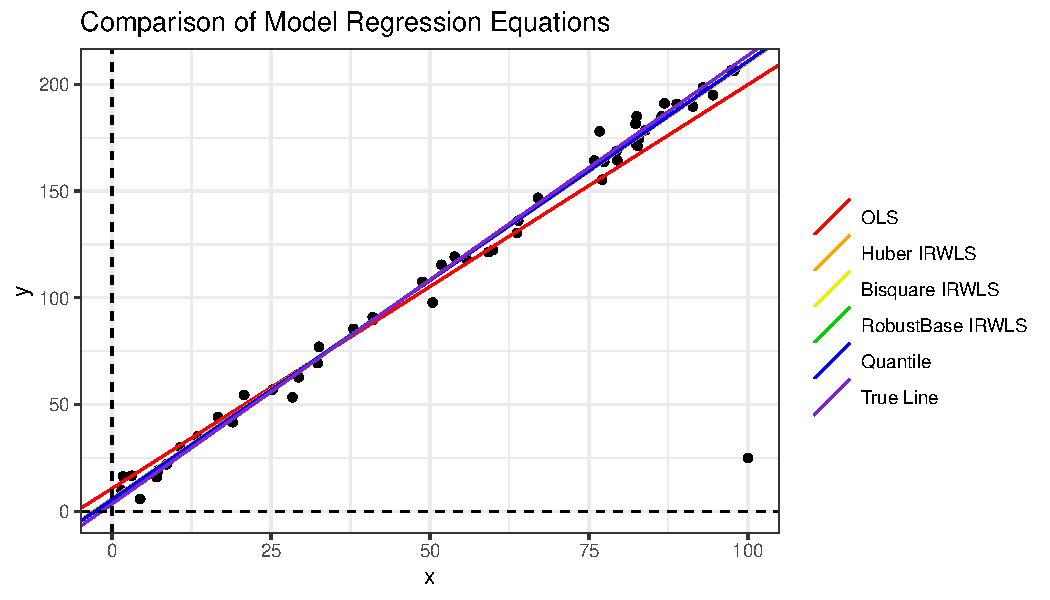
\includegraphics[width=\maxwidth]{figure/unnamed-chunk-34-1} 
\end{knitrout}


\label{all.models.plot}
\caption{Scatterplot of the Data and Each Model}

\end{figure}

\textcolor{red}{When comparing all of the models visually, the only one that stands out is the standard OLS model, with very little variation amongst the true line and the robust methods.}

\begin{knitrout}\scriptsize
\definecolor{shadecolor}{rgb}{0.969, 0.969, 0.969}\color{fgcolor}\begin{kframe}
\begin{alltt}
\hldef{total_sum} \hlkwb{<-} \hlkwd{tibble}\hldef{(}\hlkwc{Method} \hldef{=} \hlkwd{c}\hldef{(}\hlsng{"OLS"}\hldef{,}
                               \hlsng{"Huber IRWLS"}\hldef{,}
                               \hlsng{"Bisquare IRWLS"}\hldef{,}
                               \hlsng{"RobustBase IRWLS"}\hldef{,}
                               \hlsng{"Quantile"}\hldef{,}
                               \hlsng{"True Values"}\hldef{),}
                    \hlkwc{Intercept} \hldef{=} \hlkwd{c}\hldef{(second_sum}\hlopt{$}\hldef{Estimate[}\hlnum{1}\hldef{],}
                                  \hldef{IWH_sum}\hlopt{$}\hldef{Estimate[}\hlnum{1}\hldef{],}
                                  \hldef{IWB_sum}\hlopt{$}\hldef{Estimate[}\hlnum{1}\hldef{],}
                                  \hldef{rob_sum}\hlopt{$}\hldef{Estimate[}\hlnum{1}\hldef{],}
                                  \hldef{quant_sum}\hlopt{$}\hldef{Estimate[}\hlnum{1}\hldef{],}
                                  \hlnum{3.5}\hldef{),}
                    \hlkwc{Slope} \hldef{=} \hlkwd{c}\hldef{(second_sum}\hlopt{$}\hldef{Estimate[}\hlnum{2}\hldef{],}
                                  \hldef{IWH_sum}\hlopt{$}\hldef{Estimate[}\hlnum{2}\hldef{],}
                                  \hldef{IWB_sum}\hlopt{$}\hldef{Estimate[}\hlnum{2}\hldef{],}
                                  \hldef{rob_sum}\hlopt{$}\hldef{Estimate[}\hlnum{2}\hldef{],}
                                  \hldef{quant_sum}\hlopt{$}\hldef{Estimate[}\hlnum{2}\hldef{],}
                                  \hlnum{2.1}\hldef{))}

\hldef{total_sum} \hlkwb{<-} \hldef{total_sum |>}
  \hlkwd{mutate}\hldef{(}\hlsng{"Intercept Error"} \hldef{= Intercept} \hlopt{-} \hldef{total_sum}\hlopt{$}\hldef{Intercept[}\hlnum{6}\hldef{],}
         \hlsng{"Slope Error"} \hldef{= Slope} \hlopt{-} \hldef{total_sum}\hlopt{$}\hldef{Slope[}\hlnum{6}\hldef{])}

\hldef{total_sum} \hlkwb{<-} \hldef{total_sum[,}\hlkwd{c}\hldef{(}\hlnum{1}\hldef{,}\hlnum{2}\hldef{,}\hlnum{4}\hldef{,}\hlnum{3}\hldef{,}\hlnum{5}\hldef{)]}

\hldef{total_sum} \hlkwb{<-} \hlkwd{xtable}\hldef{(total_sum,}
                    \hlkwc{label} \hldef{=} \hlsng{"total.model.sum"}\hldef{,}
                    \hlkwc{caption} \hldef{=} \hlsng{"Comparison of Each Model"}\hldef{,}
                    \hlkwc{digits} \hldef{=} \hlnum{3}\hldef{)}
\end{alltt}
\end{kframe}
\end{knitrout}


% latex table generated in R 4.5.1 by xtable 1.8-4 package
% Fri Nov 21 10:34:06 2025
\begin{table}[H]
\centering
\begingroup\normalsize
\begin{tabular}{lrrrr}
  \hline
Method & Intercept & Intercept Error & Slope & Slope Error \\ 
  \hline
OLS & 10.742 & 7.242 & 1.891 & -0.209 \\ 
  Huber IRWLS & 6.039 & 2.539 & 2.042 & -0.058 \\ 
  Bisquare IRWLS & 5.702 & 2.202 & 2.050 & -0.050 \\ 
  RobustBase IRWLS & 5.633 & 2.133 & 2.052 & -0.048 \\ 
  Quantile & 5.529 & 2.029 & 2.053 & -0.047 \\ 
  True Values & 3.500 & 0.000 & 2.100 & 0.000 \\ 
   \hline
\end{tabular}
\endgroup
\caption{Comparison of Each Model} 
\label{total.model.sum}
\end{table}


\textcolor{red}{Likely coincidentally, each successive model we tested is closer to the true value than the last, with the biggest difference being after we moved from OLS to the robust methods.}


  %%%%%%%%%%%%%%%%%%%%%%%%%%%%%%%%%%%%%%%%%%%%%%%%%%%%%%%%%%%%%%%%%%%%%%%%%%%%%%
  %%%%%%%%%%%%%%%%%%%%%%%%%%%%%%%%%%%%%%%%%%%%%%%%%%%%%%%%%%%%%%%%%%%%%%%%%%%%%%
  % Question 5
  %%%%%%%%%%%%%%%%%%%%%%%%%%%%%%%%%%%%%%%%%%%%%%%%%%%%%%%%%%%%%%%%%%%%%%%%%%%%%%
  %%%%%%%%%%%%%%%%%%%%%%%%%%%%%%%%%%%%%%%%%%%%%%%%%%%%%%%%%%%%%%%%%%%%%%%%%%%%%%
\item \textbf{Optional, but recommended} Complete Questions 3-4, but use $n=1000$.
What changes? Why do you think that is?

\end{enumerate}
\bibliography{bib}
\end{document}

